\begin{definition}
Пусть $E_1, E_2$~--- линейные нормированные пространства,
$A \in \mathcal{L}(E_1, E_2)$. \textit{Сопряжённым} к оператору $A$ называется
$A^*\!\!:\: E_2^* \to E_1^*$, определённый по правилу
$\forall g \in E_2^* \left((A^* g)(x) = g(A x) \right)$.  

\end{definition}
\begin{figure}[H]
\centering
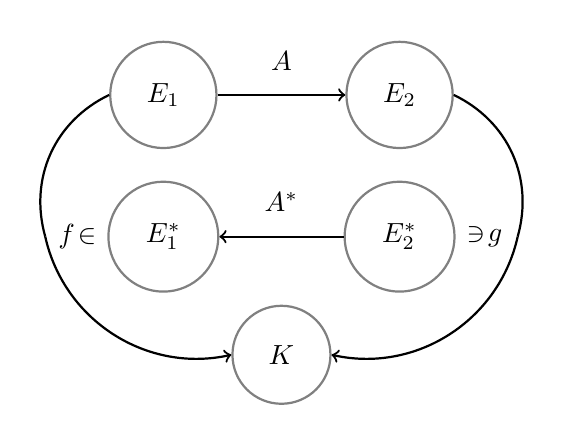
\begin{tikzpicture}[inner sep=3mm,thick]
  \node (field) at (0,0) [circle,draw=black!50] {\(\mathbb{K}\)};
  \node (E1_conj) at (-1.5,1.5) [circle,draw=black!50,label=left:\(f\! \in\!\!\!\)] {\(E_1^*\)};
  \node (E1) at (-1.5,3.3) [circle,draw=black!50] {\(E_1\)};
  \node (E2_conj) at (1.5,1.5) [circle,draw=black!50,label=right:\(\!\!\!\ni\! g\)] {\(E_2^*\)};
  \node (E2) at (1.5,3.3) [circle,draw=black!50] {\(E_2\)};
  \draw [-,bend right=40] (E1.west) to (-3,1.5);
  \draw [->,bend right=45] (-3,1.5) to (field.west);
  \draw [-,bend left=40] (E2.east) to (3,1.5);
  \draw [->,bend left=45] (3,1.5) to (field.east);
  \draw [->] (E1) to node[above] {\(A\)} (E2);
  \draw [->] (E2_conj) to node[above] {\(A^*\)} (E1_conj);

% Версия с прямыми стрелками
  % \node (field) at (0,0) [circle,draw=black!50] {\(\mathbb{K}\)};
  % \node (E1_conj) at (-1.5,1.5) [circle,draw=black!50,label=left:\(f\: \in\!\)] {\(E_1^*\)};
  % \node (E1) at (-1.5,3.3) [circle,draw=black!50] {\(E_1\)};
  % \node (E2_conj) at (1.5,1.5) [circle,draw=black!50,label=right:\(\!\ni\: g\)] {\(E_2^*\)};
  % \node (E2) at (1.5,3.3) [circle,draw=black!50] {\(E_2\)};
  % \draw [-,bend right=45] (E1.west) to (-3.6,1.5);
  % \draw [-,bend right=45] (-3.6,1.5) to (-2.1,0);
  % \draw [->] (-2.1,0) to (field.west);
  % \draw [-,bend left=45] (E2.east) to (3.6,1.5);
  % \draw [-,bend left=45] (3.6,1.5) to (2.1,0);
  % \draw [->] (2.1,0) to (field.east);
  % \draw [->] (E1) to node[above] {\(A\)} (E2);
  % \draw [->] (E2_conj) to node[above] {\(A^*\)} (E1_conj);
\end{tikzpicture}
\end{figure}



\begin{theorem}[9.1]
    Пусть $E_1, E_2$~--- линейные нормированные пространства. Тогда $\forall A \in \mathcal{L}(E_1, E_2) \; \exists ! A^*$, причём $\| A^* \| =\| A\|$
\end{theorem}
\begin{proof}
    Существование и единственность очевидны из определения.
    Ограниченность оператора $A^*$: (модуль т.к. линейный функционал действует в поле $\K$)

    \[
    |(A^*g)(x)| = |g(Ax)| \leqslant \|g\| \cdot \|Ax\| \leqslant
    \|g\| \cdot \|A\| \cdot \|x\|
    \]

    Перейдем к супремуму по $\|x\|=1$
    \[
    \|A^* g\| \leqslant \|A\|  \cdot \|g\|  \; \Rightarrow \;
    \|A^*\| \leqslant \|A\|
    \]
    % кухня Хана-Банаха
    С другой стороны, $\|A\| \leqslant \|A^*\|$, так как по следствию~\nameref{hbcorollary4} теоремы Хана--Банаха
    \[ \| Ax\| = \sup_{\|g\|_{E_2^*} = 1} |g(Ax)| = 
    \sup_{\|g\|_{E_2^*}=1} |(A^*g)(x)| \leqslant  \sup_{\|g\|_{E_2^*}=1} \|g\|  \|A^*\| \|x\| = \|A^*\| \|x\| \]
\end{proof}

\begin{unnecessary}
    \begin{theorem}[9.3 (б/д)]
    Пусть $E_1, E_2$~--- линейные нормированные пространства. Тогда
    $\exists A^{-1} \in \mathcal{L}(E_2, E_1)$ тогда и только тогда, когда
    $\exists (A^*)^{-1} \in \mathcal{L}(E_1^*, E_2^*)$.
    При этом $(A^*)^{-1} = (A^{-1})^*$.
    \end{theorem}
\end{unnecessary}

